\documentclass[12pt]{beamer}
\usepackage{../Estilos/BeamerFC}
\usepackage{tabulary}
\usepackage{../Estilos/ColoresLatex}
\usepackage{courier}
\usepackage{listingsutf8}
\usepackage{listings}
\usepackage{xcolor}
\usepackage{textcomp}
\usepackage{color}
\definecolor{deepblue}{rgb}{0,0,0.5}
\definecolor{brown}{rgb}{0.59, 0.29, 0.0}
\definecolor{OliveGreen}{rgb}{0,0.25,0}
% \usepackage{minted}

\DeclareCaptionFont{white}{\color{white}}
\DeclareCaptionFormat{listing}{\colorbox{gray}{\parbox{0.98\textwidth}{#1#2#3}}}
\captionsetup[lstlisting]{format=listing,labelfont=white,textfont=white}
\renewcommand{\lstlistingname}{Código}


\definecolor{Code}{rgb}{0,0,0}
\definecolor{Keywords}{rgb}{255,0,0}
\definecolor{Strings}{rgb}{255,0,255}
\definecolor{Comments}{rgb}{0,0,255}
\definecolor{Numbers}{rgb}{255,128,0}

\makeatletter

\newif\iffirstchar\firstchartrue
\newif\ifstartedbyadigit
\newif\ifprecededbyequalsign

\newcommand\processletter
{%
  \ifnum\lst@mode=\lst@Pmode%
    \iffirstchar%
        \global\startedbyadigitfalse%
      \fi
      \global\firstcharfalse%
    \fi
}

\newcommand\processdigit
{%
  \ifnum\lst@mode=\lst@Pmode%
      \iffirstchar%
        \global\startedbyadigittrue%
      \fi
      \global\firstcharfalse%
  \fi
}

\lst@AddToHook{OutputOther}%
{%
  \lst@IfLastOtherOneOf{=}
    {\global\precededbyequalsigntrue}
    {}%
}

\lst@AddToHook{Output}%
{%
  \ifprecededbyequalsign%
      \ifstartedbyadigit%
        \def\lst@thestyle{\color{orange}}%
      \fi
    \fi
  \global\firstchartrue%
  \global\startedbyadigitfalse%
  \global\precededbyequalsignfalse%
}

\lstset{ 
language=Python,                % choose the language of the code
basicstyle=\footnotesize\ttfamily,       % the size of the fonts that are used for the code
numbers=left,                   % where to put the line-numbers
numberstyle=\scriptsize,      % the size of the fonts that are used for the line-numbers
stepnumber=1,                   % the step between two line-numbers. If it is 1 each line will be numbered
numbersep=5pt,                  % how far the line-numbers are from the code
backgroundcolor=\color{white},  % choose the background color. You must add \usepackage{color}
showspaces=false,               % show spaces adding particular underscores
showstringspaces=false,         % underline spaces within strings
showtabs=false,                 % show tabs within strings adding particular underscores
frame=single,   		% adds a frame around the code
tabsize=2,  		% sets default tabsize to 2 spaces
captionpos=t,   		% sets the caption-position to bottom
breaklines=true,    	% sets automatic line breaking
breakatwhitespace=false,    % sets if automatic breaks should only happen at whitespace
escapeinside={| |},  % if you want to add a comment within your code
stringstyle =\color{OliveGreen},
otherkeywords={as, np.array, np.concatenate, np.linspace, linspace, interpolate.interp1d, kind, plt.plot, .copy, np.arange, np.cos, np.pi, lw, ls, label, splrep, splev, plt.legend, loc, plt.title, plt.ylim, plt.show, sign, math.ceil, math.log, np.sqrt, np.exp, np.zeros, plt.xlabel, plt.ylabel, plt.xlim, np.identity, random, np.dot, np.outer, np.diagonal },             % Add keywords here
keywordstyle = \color{blue},
commentstyle = \color{darkcerulean},
identifierstyle = \color{black},
literate=%
         {á}{{\'a}}1
         {é}{{\'e}}1
         {í}{{\'i}}1
         {ó}{{\'o}}1
         {ú}{{\'u}}1
%
%keywordstyle=\ttb\color{deepblue}
%fancyvrb = true,
}

\lstdefinestyle{FormattedNumber}{%
    literate={0}{{\textcolor{red}{0}}}{1}%
             {1}{{\textcolor{red}{1}}}{1}%
             {2}{{\textcolor{red}{2}}}{1}%
             {3}{{\textcolor{red}{3}}}{1}%
             {4}{{\textcolor{red}{4}}}{1}%
             {5}{{\textcolor{red}{5}}}{1}%
             {6}{{\textcolor{red}{6}}}{1}%
             {7}{{\textcolor{red}{7}}}{1}%
             {8}{{\textcolor{red}{8}}}{1}%
             {9}{{\textcolor{red}{9}}}{1}%
             {.0}{{\textcolor{red}{.0}}}{2}% Following is to ensure that only periods
             {.1}{{\textcolor{red}{.1}}}{2}% followed by a digit are changed.
             {.2}{{\textcolor{red}{.2}}}{2}%
             {.3}{{\textcolor{red}{.3}}}{2}%
             {.4}{{\textcolor{red}{.4}}}{2}%
             {.5}{{\textcolor{red}{.5}}}{2}%
             {.6}{{\textcolor{red}{.6}}}{2}%
             {.7}{{\textcolor{red}{.7}}}{2}%
             {.8}{{\textcolor{red}{.8}}}{2}%
             {.9}{{\textcolor{red}{.9}}}{2}%
             {\ }{{ }}{1}% handle the space
         ,%
          %mathescape=true
          escapeinside={__}
          }



\usetheme{Warsaw}
\usecolortheme{seahorse}
%\useoutertheme{default}
\setbeamercovered{invisible}
% or whatever (possibly just delete it)
\setbeamertemplate{section in toc}[sections numbered]
\setbeamertemplate{subsection in toc}[subsections numbered]
\setbeamertemplate{subsection in toc}{\leavevmode\leftskip=3.2em\rlap{\hskip-2em\inserttocsectionnumber.\inserttocsubsectionnumber}\inserttocsubsection\par}
\setbeamercolor{section in toc}{fg=blue}
\setbeamercolor{subsection in toc}{fg=blue}
\setbeamercolor{frametitle}{fg=blue}
\setbeamertemplate{caption}[numbered]

\setbeamertemplate{footline}
\beamertemplatenavigationsymbolsempty
\setbeamertemplate{headline}{}


\makeatletter
\setbeamercolor{section in foot}{bg=gray!30, fg=black!90!orange}
\setbeamercolor{subsection in foot}{bg=blue!30}
\setbeamercolor{date in foot}{bg=black}
\setbeamertemplate{footline}
{
  \leavevmode%
  \hbox{%
  \begin{beamercolorbox}[wd=.333333\paperwidth,ht=2.25ex,dp=1ex,center]{section in foot}%
    \usebeamerfont{section in foot} \insertsection
  \end{beamercolorbox}%
  \begin{beamercolorbox}[wd=.333333\paperwidth,ht=2.25ex,dp=1ex,center]{subsection in foot}%
    \usebeamerfont{subsection in foot}  \insertsubsection
  \end{beamercolorbox}%
  \begin{beamercolorbox}[wd=.333333\paperwidth,ht=2.25ex,dp=1ex,right]{date in head/foot}%
    \usebeamerfont{date in head/foot} \insertshortdate{} \hspace*{2em}
    \insertframenumber{} / \inserttotalframenumber \hspace*{2ex} 
  \end{beamercolorbox}}%
  \vskip0pt%
}
\makeatother

\makeatletter
\patchcmd{\beamer@sectionintoc}{\vskip1.5em}{\vskip0.8em}{}{}
\makeatother

%\newlength{\depthofsumsign}
%\setlength{\depthofsumsign}{\depthof{$\sum$}}
% \newcommand{\nsum}[1][1.4]{% only for \displaystyle
%     \mathop{%
%         \raisebox
%             {-#1\depthofsumsign+1\depthofsumsign}
%             {\scalebox
%                 {#1}
%                 {$\displaystyle\sum$}%
%             }
%     }
% }
\def\scaleint#1{\vcenter{\hbox{\scaleto[3ex]{\displaystyle\int}{#1}}}}
\def\scaleoint#1{\vcenter{\hbox{\scaleto[3ex]{\displaystyle\oint}{#1}}}}
\def\bs{\mkern-12mu}

%\usefonttheme{serif}

\title{\large{Tema 1 - Errores y artimética de punto flotante}}
\author{M. en C. Gustavo Contreras Mayén}
\date{ }

\begin{document}
\maketitle

\section*{Contenido}
\frame[allowframebreaks]{\frametitle{Contenido} \tableofcontents[currentsection, hideallsubsections]}

\section{Más sobre los errores}
\frame{\tableofcontents[currentsection, hideothersubsections]}
\subsection{Fuentes de error}
\begin{frame}
\frametitle{Hablando de errores}
El problema es que como científicos, queremos un resultado correcto o al menos en el que la incertidumbre sea pequeña y de tamaño conocido.
\end{frame}
\begin{frame}
\frametitle{Fuentes de errores computacionales}
Existen al menos cuatro fuentes de errores que se pueden presentar en los cálculos computacionales:
\pause
\setbeamercolor{item projected}{bg=asparagus,fg=arsenic}
\setbeamertemplate{enumerate items}{%
\usebeamercolor[bg]{item projected}%
\raisebox{1.5pt}{\colorbox{bg}{\color{fg}\footnotesize\insertenumlabel}}%
}
\begin{enumerate}[<+->]
\item Un modelo equivocado.
\item Errores aleatorios.
\item Errores por aproximación
\item Errores por redondeo.
\end{enumerate}
\end{frame}

\subsection{Errores aleatorios}

\begin{frame}
\frametitle{Errores aleatorios}
Se presenta una imprecisión debida por acontecimientos tales como: fluctuaciones en la electrónica, incidencia de rayos cósmicos, o alguien que se tropieza con un enchufe.
\\
\bigskip
\pause
Éstos errores pueden ser raros, pero no tenemos ningún control sobre ellos y su probabilidad aumenta conforme transcurre el tiempo.
\end{frame}

\subsection{Errores por aproximación}

\begin{frame}
\frametitle{Errores por aproximación}
La imprecisión surge de la simplificación de las matemáticas para que un problema pueda ser resuelto en la computadora.
\\
\bigskip
\pause
Incluyen la sustitución de series infinitas por sumas finitas, intervalos infinitesimales por finitos, y funciones variables por constantes.
\end{frame}
\begin{frame}
\frametitle{Errores por aproximación}
Por ejemplo:
\pause
\begin{eqnarray}
\begin{aligned}[b]
\sin(x) &= \nsum_{n = 1}^{\infty} \: \dfrac{(-1)^{n-1} \: x^{2n - 1}}{(2n - 1)!} \hspace{0.5cm} \text{(exacta)} \\[5pt] \pause
& \simeq \nsum_{n = 1}^{N} \: \dfrac{(-1)^{n-1} \: x^{2n - 1}}{(2n - 1)!} \hspace{0.5cm} \text{(aproximación)} \pause \\[5pt] \pause
& = \sin(x) + \varepsilon(x, N)
\end{aligned}
\label{eq:ecuacion_02_02}
\end{eqnarray}
\pause
donde $\varepsilon(x,N)$ es el error por la aproximación, en este caso $\varepsilon$ corresponde a los términos desde $N + 1$ a $\infty$.
\end{frame}
\begin{frame}
\frametitle{Errores por aproximación}
Dado que el error por la aproximación se genera en el algoritmo que usamos para aproximar la matemática, también se le conoce como \underline{error del algoritmo}.
\end{frame}
\begin{frame}
\frametitle{Errores por aproximación}
Para una buena y razonable aproximación, el error debido por la aproximación debería de reducirse cuando el valor de $N$ se incrementa, y debería de anularse en el límite $N \rightarrow \infty$.
\end{frame}
\begin{frame}
\frametitle{Errores por aproximación}
Para el ejemplo (\ref{eq:ecuacion_02_02}), como la escala de $N$ se fija por el valor de $x$, un pequeño error de aproximación requiere que $ N \geqslant x$.
\\
\bigskip
\pause
Por lo que si $x$ y $N$ son valores cercanos entre sí, el error de aproximación será grande.
\end{frame}

\subsection{Errores por redondeo}

\begin{frame}
\frametitle{Errores por redondeo}
La imprecisión se genera por el número finito de dígitos utilizados para almacenar números de punto flotante.
\\
\bigskip
\pause
Estos \enquote{errores} son análogos a la incertidumbre en la medición de una cantidad física encontrada en un laboratorio de física.
\end{frame}
\begin{frame}
\frametitle{Errores por redondeo}
El error general de redondeo se acumula a medida que el equipo maneja más números, es decir, a medida que aumenta el número de pasos en un cálculo, y puede hacer que algunos algoritmos se vuelvan inestables con un rápido aumento del error.
\end{frame}
\begin{frame}
\frametitle{Errores por redondeo}
En algunos casos, el error por redondeo puede convertirse en el componente principal en la respuesta, lo que lleva a lo que los expertos informáticos llaman \textocolor{ao}{basura}.
\end{frame}
\begin{frame}
\frametitle{Errores por redondeo}
Por ejemplo, si la computadora mantiene cuatro decimales, entonces almacenará $\frac{1}{3}$ como $0.3333$ y $\frac{2}{3} = 0.6667$, donde el equipo ha \enquote{redondeado} el último dígito en $\dfrac{2}{3}$.
\end{frame}
\begin{frame}
\frametitle{Errores por redondeo}
Por consiguiente, si hacemos en la computadora un cálculo tan simple como $2 \frac{1}{3} - \frac{2}{3}$, produce:
\pause
\begin{equation}
2 \left( \dfrac{1}{3} \right) - \dfrac{2}{3} = 0.6666 - 0.6667 = -0.0001 \neq 0
\label{eq:ecuacion_02_03}
\end{equation}
\pause
Aunque el resultado es pequeño, no es $0$, y si se repite este cálculo varios millones de veces, \pause la respuesta final puede que ni siquiera sea pequeña (\textocolor{lava}{la basura genera basura}).
\end{frame}

\section{Modelos para el desastre}
\frame{\tableofcontents[currentsection, hideothersubsections]}
\subsection{Definiciones}

\begin{frame}[fragile]
\frametitle{Definiciones}
Sea $x$ el valor exacto de una cierta cantidad y $x^{*}$ la aproximación a esa cantidad.
\\
\bigskip
\pause
Por definición, el valor absoluto asociado a $x$ es:
\pause
\begin{equation}
\Delta = \abs{ x - x^{*} } 
\label{eq:ecuacion_01_03}	
\end{equation}
\end{frame}
\begin{frame}
\frametitle{Definiciones}
En general, los cálculos numéricos operan con aproximaciones tanto a las cantidades como a sus errores absolutos.
\\
\bigskip
\pause
En el caso ideal, en el que, además de la aproximación $x$, también se conocería el error absoluto exacto, el número exacto sería exactamente expresable como:
\pause
\begin{equation}
x = x^{*} \pm \Delta^{*}
\label{eq:ecuacion_01_04}    	
\end{equation}    
\end{frame}
\begin{frame}
\frametitle{Definiciones}
Sin embargo, en general, solo está disponible una estimación del error absoluto y, en consecuencia, solo un estimado del valor exacto puede determinarse:
\pause
\begin{equation}
x^{*} - \Delta \leq x \leq x^{*} + \Delta
\label{eq:ecuacion_01_05}
\end{equation}
\end{frame}
\begin{frame}
\frametitle{Definiciones}
Para que la estimación $x^{*}$ sea confiable, es importante que $\Delta$ no subestime el error verdadero, es decir, $\Delta \geq \Delta^{*}$, en este caso, se denomina \emph{limitación de error absoluto}.
\end{frame}
\begin{frame}
\frametitle{Más definiciones}
El error relativo $\delta^{*}$ es la aproximación de $x^{*}$ a $x$, y es igual al cociente del error absoluto con el número exacto:
\pause
\begin{equation}
\delta^{*} = \dfrac{\Delta^{*}}{\abs{x}} \hspace{1cm} x \neq 0
\label{eq:ecuacion_01_06}
\end{equation}
\end{frame}
\begin{frame}
\frametitle{Más definiciones}
Re-emplazando $\Delta^{*}$ en la ecuación(\ref{eq:ecuacion_01_04}) de la ecuación (\ref{eq:ecuacion_01_06}), tendremos la expresión para un número exacto:
\pause
\begin{equation}
x \simeq x^{*} \: (1 \pm \delta^{*})
\label{eq:ecuacion_01_07}
\end{equation}
\end{frame}
\begin{frame}
\frametitle{Más definiciones}
Basándose en el error relativo de la aproximación $\delta \geq \delta^{*}$, se expresa el valor exacto como:
\begin{equation}
x \simeq x^{*} \: (1 \pm \delta)
\label{eq:ecuacion_01_08}
\end{equation}
\end{frame}

\section{Errores en las op. aritméticas}
\frame{\tableofcontents[currentsection, hideothersubsections]}
\subsection{Errores en las op. elementales}

\begin{frame}
\frametitle{Errores en las operaciones elementales}
Revisaremos la forma en que varias operaciones elementales propagan los errores relativos de sus operandos.
\\
\bigskip
\pause
En relación con los cálculos numéricos, las consideraciones desarrolladas a continuación se refieren específicamente a los errores de redondeo y truncamiento.
\end{frame}

\subsection{Error en la suma}

\begin{frame}
\frametitle{Error en la suma}
Sea la suma de dos números próximos, $x_{1}$ y $x_{2}$, que tienen el mismo signo.
\\
\bigskip
\pause
La suma evidentemente conserva el signo y acumula las magnitudes de los operandos:
\pause
\begin{equation}
x = x_{1} + x_{2}
\label{eq:ecuacion_01_14}
\end{equation}
\end{frame}
\begin{frame}
\frametitle{Error en la suma}
Tenemos que el error total es:
\begin{align*}
\Delta x =  \Delta x_{1} + \Delta x_{2}
\end{align*}
\pause
pero, dado que los errores individuales pueden, en función de sus signos, compensarse mutuamente y acumularse.
\end{frame}
\begin{frame}
\frametitle{Error en la suma}
La suma de los errores absolutos de los operandos proporciona en realidad un límite superior para el error absoluto total de la suma:
\begin{equation}
\Delta \leq \Delta_{1} + \Delta_{2}
\label{eq:ecuacion_01_15}
\end{equation}
\end{frame}
\begin{frame}
\frametitle{Error relativo en la suma}
El error relativo de la suma de dos números proximos del mismo signo no supera el error relativo más grande de los sumandos:
\pause
\begin{equation}
\delta \leq \max{(\delta_{1}, \delta_{2})}
\label{eq:ecuacion_01_16}
\end{equation}
\end{frame}

\subsection{Error en la diferencia}

\begin{frame}
\frametitle{Error en la diferencia}
Ahora consideremos la diferencia de dos números próximos con \emph{el mismo signo}:
\pause
\begin{equation}
x = x_{1} - x_{2}
\label{eq:ecuacion_01_18}
\end{equation}
\pause
Debería ser evidente que las ecuaciones (\ref{eq:ecuacion_01_14}) y (\ref{eq:ecuacion_01_18}) cubren todas las posibles situaciones algebraicas.
\end{frame}
\begin{frame}
\frametitle{Error en la diferencia}
Al igual que en el caso de la suma, el caso más desfavorable es aquél en el que los errores absolutos se potencian entre sí, y, por lo tanto, la suma de los errores absolutos es, de nuevo, el límite superior para el error absoluto de la diferencia:
\pause
\begin{align*}
\Delta \leq  \Delta_{1} + \Delta_{2}
\end{align*}
\end{frame}
\begin{frame}
\frametitle{Error en la diferencia}
Maximizando el error absoluto total en la definición de error relativo ($\delta$), tenemos que:
\pause
\begin{equation}
\delta \leq \dfrac{\Delta_{1} + \Delta_{2}}{\abs{x_{1} - x_{2}}} = \dfrac{\abs{x_{1}} \: \delta_{1} + \abs{x_{2}} \: \delta_{2}}{\abs{x_{1} - x_{2}}}
\end{equation}
\end{frame}
\begin{frame}
\frametitle{Error en la diferencia}
Si los sumandos están cerca de su valor, la diferencia absoluta $\abs{x_{1} - x_{2}}$ es pequeño e, incluso para pequeños errores relativos individuales, $\delta_{1}$ y $\delta_{2}$, el error relativo de la diferencia, $\delta$, puede volverse significativo.
\end{frame}

\subsection{Error en el producto}

\begin{frame}
\frametitle{Error en el producto}
El error relativo de un producto de dos números próximos $x = x_{1} \: x_{2}$, no excede a la suma del error relativo de los factores $\delta_{1}$ y $\delta_{2}$:
\pause
\begin{equation}
\delta = \delta_{1} + \delta_{2}
\label{eq:ecuacion_01_20}
\end{equation}
\end{frame}

\subsection{Error en el cociente}

\begin{frame}
\frametitle{Error en el cociente}
Consideremos ahora el cociente:
\begin{align*}
x = \dfrac{x_{1}}{x_{2}}
\end{align*}
de dos números próximos no nulos.
\\
\bigskip
\pause
Teniendo en cuenta, una vez más, que $x_{1}$ y $x_{2}$ se ven afectados por pequeños errores absolutos $\Delta_{1} = \abs{\Delta x_{1}}$ y $\Delta_{2} = \abs{\Delta x_{2}}$:
\end{frame}
\begin{frame}
\frametitle{Error en el cociente}
Obtenemos la relación límite:
\pause
\begin{equation}
\delta = \delta_{1} + \delta_{2}
\label{eq:ecuacion_01_27}
\end{equation}
que establece que el error relativo del cociente no excede los errores relativos acumulados del dividendo y divisor.
\end{frame}

\section{Ejercicios}
\frame{\tableofcontents[currentsection, hideothersubsections]}
\subsection{Aproximando con una serie}

\begin{frame}
\frametitle{Retomando el problema}
Veamos el resultado y su error al hacer una aproximación de la expresión:
\pause
\begin{align*}
\sin(x) \simeq \nsum_{n = 1}^{N} \: \dfrac{(-1)^{n-1} \: x^{2n-1}}{(2 \, n - 1)!}
\end{align*}
\end{frame}
\begin{frame}
\frametitle{Punto importante}
No perdamos de vista que la anterior expresión nos indica que debemos de calcular $(-1)^{n-1} \: x^{2n-1}$, \pause para luego dividirlo entre $(2 \, n - 1)!$.
\\
\bigskip
\pause
No es una buena idea para implementarla en el código.
\end{frame}
\begin{frame}
\frametitle{Punto importante}
Para valores grandes de $n$:
\setbeamercolor{item projected}{bg=bananayellow,fg=bistre}
\setbeamertemplate{enumerate items}{%
\usebeamercolor[bg]{item projected}%
\raisebox{1.5pt}{\colorbox{bg}{\color{fg}\footnotesize\insertenumlabel}}%
}
\begin{enumerate}[<+->]
\item Calcular el factorial puede consumir demasiado tiempo.
\item Elevar a la potencia, puede causar un \textocolor{ao}{overflow}, y como es el denominador, no queremos problemas en esta parte.
\end{enumerate}
\end{frame}
\begin{frame}
\frametitle{Cambiando el cálculo}
Cambiemos la operación de la siguiente manera: \pause usaremos una multiplicación que nos relacione el \emph{\textocolor{blue-violet}{siguiente término}} con un \emph{\textocolor{burgundy}{término previo}} de la serie.
\end{frame}
\begin{frame}
\frametitle{Relación entre los términos}
\begin{eqnarray*}
\begin{aligned}
\dfrac{(-1)^{n-1} \, x^{2n-1}}{(2 \, n - 1)!} &= \dfrac{-x^{2}}{(2 \, n - 1)(2 \, n -2)} \, \dfrac{(-1)^{n-2} \, x^{2n-3}}{(2 \, n - 3)!} \\[1em] \pause
\Rightarrow \hspace{0.2cm} n \, \text{término} &= \dfrac{-x^{2}}{(2 \, n - 1)(2 \, n -2)} \, (n - 1) \, \text{término}
\end{aligned}
\end{eqnarray*}
\end{frame}
\begin{frame}
\frametitle{Primera propuesta de código}
Implementemos una primera propuesta de código, que luego de revisarla tendrá una mejora.
\end{frame}
\begin{frame}
\frametitle{¿Qué es lo que hará el código?}
Debemos de introducir un valor $x$ de tal manera que se evalúe con la suma finita, toma en cuenta que la función \funcionazul{math.sin(x)}, el argumento $x$ debe de estar en radianes.
\\
\bigskip
\pause
Podemos hacer la conversión conocida de la geometría, \pause o utilizar la función \funcionazul{math.radians(x)} para obtener el valor en radianes.
\end{frame}
\begin{frame}
\frametitle{¿Qué es lo que hará el código?}
Luego vamos a calcular el error relativo (con una función de usuario), ocupando como valor \enquote{exacto} el que nos devuelve la función \funcionazul{math.sin(x)} de \python.
\\
\bigskip
\pause
Usemos el valor de $x = \SI{30}{\degree}$ para el ejercicio.
\end{frame}
\begin{frame}[allowframebreaks, fragile]
\frametitle{Primera propuesta de código}
\begin{lstlisting}[caption=Código para aproximar sen(x)]
import math

# Aqui va la funcion para el error relativo
# def funcion(arg1, arg2):
#     codigo necesario


a = float(input('Teclea el valor a evaluar: '))
x = math.radians(a)

j = 0
n = 10
suma = x
term =  x

print('x \t aproximacion \t  error')
for i in range(2, n):
    j += 1
    term = (-term * x * x)/((2 * i - 1) * (2 * i - 2))
    suma  = suma + term
    print('{0:} \t {1:1.10f} \t {2:1.5e}'.format(j, suma, error(arg1, arg2)))
\end{lstlisting}
\end{frame}
\begin{frame}
\frametitle{Resultado}
\begin{table}
\renewcommand{\arraystretch}{0.8}
\begin{tabular}{c c c}
Iteración & Aproximación & Error \\ \hline
$1$ & $0.4996741794$ & $6.51641e-02$ \\
$2$ & $0.5000021326$ & $4.26518e-04$ \\
$3$ & $0.4999999919$ & $1.62620e-06$ \\
$4$ & $0.5000000000$ & $4.05599e-09$ \\
$5$ & $0.5000000000$ & $7.12763e-12$ \\
$6$ & $0.5000000000$ & $1.11022e-14$ \\
$7$ & $0.5000000000$ & $0.00000e+00$ \\
$8$ & $0.5000000000$ & $0.00000e+00$ \\
\end{tabular}
\end{table}
\end{frame}
\begin{frame}
\frametitle{Generando una gráfica}
Para tener una mejor idea de lo que sucede, hagamos una gráfica del error relativo en cada iteración.
\\
\bigskip
\pause
La siguiente gráfica nos indica los valores obtenidos y el punto de iteración, es por ello que no se utiliza una \emph{línea continua} para unir los puntos.
\end{frame}
\begin{frame}
\frametitle{Gráfica del error relativo}
\begin{figure}
    \centering
    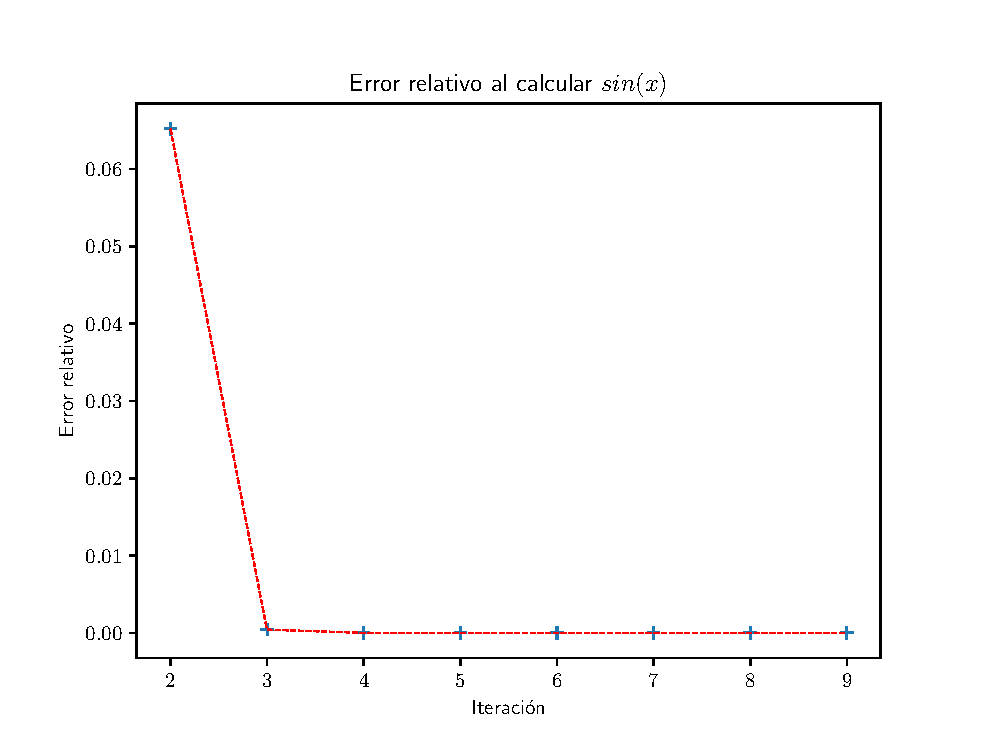
\includegraphics[scale=0.6]{Imagenes/Plot_Serie_Seno_01.eps}
\end{figure}
\end{frame}
\begin{frame}
\frametitle{Ajustando el eje $x$}
Notarás que en el eje $x$ el punto inicial está en la iteración $2$ con su correspondiente valor del error relativo, \pause para mostrarlo así en la gráfica, hay que usar una lista con los mismos puntos y ocuparla como argumento en \textocolor{ao}{matplotlib}.
\end{frame}
\begin{frame}[fragile]
\frametitle{Agregando una lista }
\begin{lstlisting}
eje_x = range(2, n)
\end{lstlisting}
Este elemento lo colocamos antes del ciclo \textocolor{ao}{for}
\end{frame}
\begin{frame}[fragile]
\frametitle{Graficando}
En la parte de graficación, anotamos lo siguiente:
\begin{lstlisting}
plt.plot(eje_x, error, '+')
plt.plot(eje_x, error)
\end{lstlisting}
De esta manera ya tendremos en el eje $x$ el valor de $2$.
\end{frame}
\begin{frame}
\frametitle{Mejorando la presentación gráfica}
Como vemos en la gráfica anterior, podemos pensar que para la segunda iteración, el error relativo se hace cero.
\\
\bigskip
\pause
Hagamos un ajuste al eje $y$, \pause hagamos el cambio a un eje logarítmico.
\end{frame}
\begin{frame}[fragile]
\frametitle{Cambiando la escala del eje}
Para cambiar la escala del eje $y$, comentamos las líneas de \textocolor{ao}{plt.plot} y hacemos uso de la función \textocolor{ao}{semilogy}:
\begin{lstlisting}
plt.semilogy(eje_x, error, '+')
plt.semilogy(eje_x, error, ls='dashed', lw=0.7, color='red')
\end{lstlisting}
\end{frame}
\begin{frame}
\frametitle{Gráfica del error relativo con eje logartímico}
\begin{figure}
    \centering
    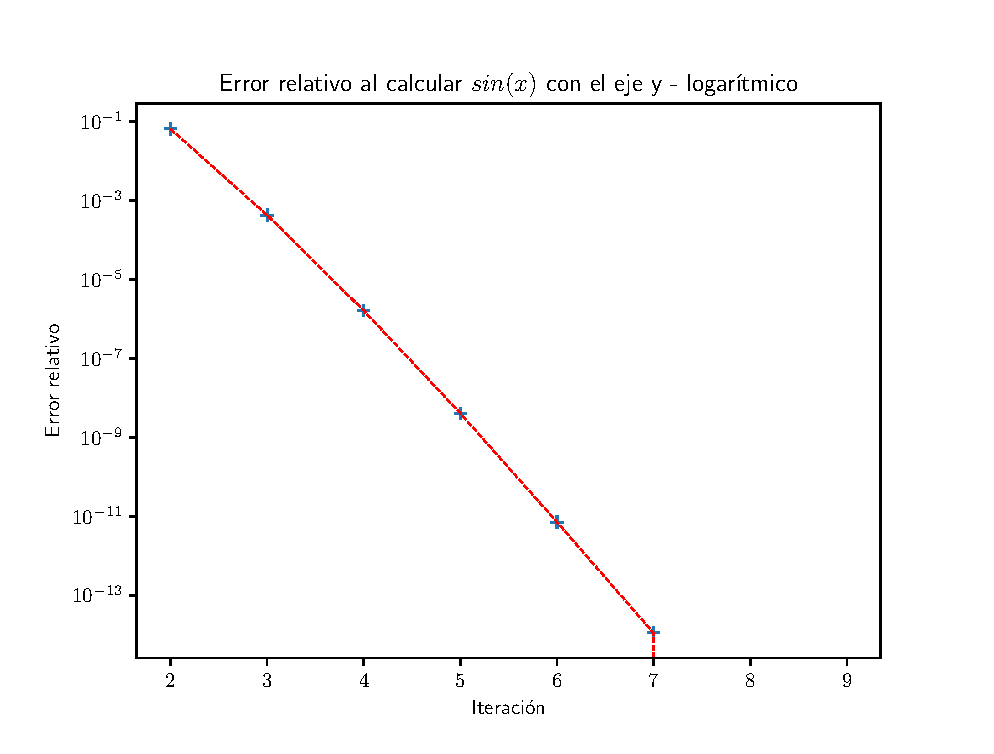
\includegraphics[scale=0.6]{Imagenes/Plot_Serie_Seno_02.eps}
\end{figure}
\end{frame}
\begin{frame}
\frametitle{Pregunta a responder}
¿Será que debemos de indicar un número \enquote{grande} de pasos para hacer que el error relativo sea muy cercano a cero?
\\
\bigskip
\pause
En el siguiente ejercicio responderemos esta pregunta.
\end{frame}

\subsection{Aproximando la derivada}

\begin{frame}
\frametitle{Errores de truncamiento}
Sabemos que este error surge de aproximar procesos continuos mediante procedimientos discretos o de procesos \enquote{infinitos} mediante procedimientos \enquote{finitos}.
\end{frame}
\begin{frame}
\frametitle{Errores de truncamiento}
Como ejemplo suele tomarse la \emph{\textocolor{ao}{diferenciación numérica}} como forma de aproximar el cálculo de una derivada en un punto (o su equivalente, la \emph{\textocolor{lilac!85!black}{integración numérica}}).
\\
\bigskip
\pause
Para el caso de discretización, el ejemplo más es usual es la utilización de métodos iterativos para resolver sistemas de ecuaciones lineales.
\end{frame}
\begin{frame}
\frametitle{Uso de una serie de Taylor}
En general, el error de truncamiento está asociado al uso de la serie de Taylor para aproximar funciones, de modo que estimar una cota del error no conlleva una dificultad mayor.
\end{frame}
\begin{frame}
\frametitle{Uso de una serie de Taylor}
Sin embargo, con el uso de la serie de Taylor suelen interactuar tanto el error inherente y/o el error de redondeo, con lo que muchas veces su influencia no es bien advertida o es muy reducida. 
\end{frame}
\begin{frame}
\frametitle{Uso de una serie de Taylor}
Veamos un ejemplo clásico: supongamos que queremos calcular una aproximación de $\pderivada{f} (x_{0})$ para una función continua, pues no es posible obtener la derivada en forma analítica o resulta muy difícil.
\\
\bigskip
\pause
Por lo tanto, usaremos un entorno del punto $x_{0}$ para calcular $\pderivada{f} (x_{0})$ utilizando solamente $f (x)$.
\end{frame}
\begin{frame}
\frametitle{Desarrollo de la serie}
Para ello nos valdremos de la serie de Taylor.
\\
\bigskip
\pause
En efecto, para cualquier punto distante $h$ de $x_{0}$ tendremos:
\pause
\begin{align*}
f (x_{0} + h) &= f(x_{0}) + \pderivada{f} (x_{0}) \, h + \sderivada{f} (x_{0}) \, \dfrac{h^{2}}{2} + \\
&+ \tderivada{f} (x_{0}) \, \dfrac{h^{3}}{6} + f^{4}(x_{0}) \dfrac{h^{4}}{24} + \ldots
\end{align*}
\end{frame}
\begin{frame}
\frametitle{Desarrollo de la serie}
Despejamos $\pderivada{f} (x_{0})$, por tanto:
\pause
\begin{align*}
\pderivada{f} (x_{0}) &= \dfrac{f (x_{0} + h) - f (x_{0})}{h} + \\
&- \left[ \sderivada{f} (x_{0}) \, \dfrac{h^{2}}{2} + \tderivada{f} (x_{0}) \, \dfrac{h^{3}}{6} + f^{4}(x_{0}) \dfrac{h^{4}}{24} + \ldots \right] 
\end{align*}
\end{frame}
\begin{frame}
\frametitle{Algoritmo propuesto}
Proponemos el siguiente algoritmo para aproximar $\pderivada{f} (x_{0})$:
\pause
\begin{align*}
\pderivada{f} (x_{0}) = \dfrac{f (x_{0} + h) - f (x_{0})}{h} + \order{h}
\end{align*}
\end{frame}
\begin{frame}
\frametitle{Error en el algoritmo propuesto}
El error que se comete en la aproximación viene dado por:
\pause
\begin{align*}
\order{h} = \left[  \sderivada{f} (x_{0}) \, \dfrac{h^{2}}{2} + \tderivada{f} (x_{0}) \, \dfrac{h^{3}}{6} + f^{4}(x_{0}) \dfrac{h^{4}}{24} + \ldots \right] 
\end{align*}
\end{frame}
\begin{frame}
\frametitle{Error por truncamiento}
El término de la derecha es el llamado \emph{error de truncamiento}, pues es lo que se truncó a la serie de Taylor para aproximar el valor buscado. 
\end{frame}
\begin{frame}
\frametitle{Velocidad de convergencia}
Este error suele asociarse también con la convergencia (o la velocidad de convergencia), que suele representarse como $\order{n}$ (generalmente, como $\order{h^{n}}$, siendo $n$ el parámetro que determina la velocidad o la convergencia. 
\end{frame}
\begin{frame}
\frametitle{Aproximación para la derivada}
En nuestro ejemplo, y dado que $h$ generalmente es menor a $1$, podemos decir que la aproximación es del tipo:
\pause
\begin{align*}
\pderivada{f} (x_{0}) = \dfrac{f (x_{0} + h) - f (x_{0})}{h} +  \order{h}
\end{align*}
\end{frame}
\begin{frame}
\frametitle{Error en la aproximación para la derivada}
En donde el error que se comete es proporcional a $h$.
\\
\medskip
\pause
Se verifica que además están los términos con $h^{2}$, $h^{3}$, etc. pero como $h < 1$ se tiene que $h^{2} \ll h$, $h^{3} \ll h^{2}$, etc. por lo que la influencia de éstos es mucho menos y despreciable.
\end{frame}
\begin{frame}
\frametitle{Primera suposición}
Supongamos por un momento que todas las derivadas $f^{i}(x_{0}) = 0$ para $i \geq 3$.
\\\
\bigskip
\pause
Entonces, tenemos que:
\begin{align*}
\left[ \pderivada{f} (x_{0}) - \dfrac{f (x_{0} + h) - f (x_{0})}{h} \right] = \dfrac{h}{2} \abs{ \sderivada{f} (\xi) }
\end{align*}
con $\xi \in [x, x + h]$
\end{frame}
\begin{frame}
\frametitle{Error al despreciar un término}
Por lo que, si conociéramos $\sderivada{f} (\xi)$ se podría acotar el error que se está cometiendo por despreciar el término $\dfrac{h}{2} \sderivada{f} (x_{0})$
\end{frame}
\begin{frame}
\frametitle{Ejercicio con la aproximación}
Como ejercicio, apliquemos el algoritmo para obtener la derivada de la función $f (x) = \sin(2 \, \pi \,  x)$ en $x_{0} = 0.45$, es decir:
\begin{align*}
\pderivada{f} (0.45) = \dfrac{\sin (2 \, \pi \, (0.45 + h)) - \sin (2 \, \pi \, 0.45)}{h}
\end{align*}
\end{frame}
\begin{frame}
\frametitle{Ejercicio con la aproximación}
Para obtener el valor de la aproximación y el error relativo en cada cálculo, implementa una función que evalúe la derivada de $f$, así como el valor del error relativo para cada $h$.
\end{frame}
\begin{frame}
\frametitle{Ejercicio con la aproximación}
Considera el valor exacto de la derivada:
\begin{align*}
\pderivada{f} (0.45) = 2 \, \pi \, \cos(2 \, \pi * 0.45) = -5.97566
\end{align*}
\end{frame}
\begin{frame}
\frametitle{Ejercicio con la aproximación}
Utiliza como valor inicial de $h = \num{d-1}$, para luego repertir el cálculo con $h = \num{d-2}$, así hasta llegar a $h = \num{d-16}$.
\\
\bigskip
\pause
Será necesario incluir una rutina de graficación para estudiar el comportamiento del error relativo.
\end{frame}
\begin{frame}
\frametitle{Construye una tabla de las aproximaciones}
\begin{table}
\renewcommand{\arraystretch}{0.9}
\centering
\begin{tabular}{l | l | l}
h & Aprox. $\pderivada{f} (x_{0})$ & Error relativo\\ \hline
$\num{d-1}$ & & \\ \hline
$\num{d-2}$ & & \\ \hline
$\num{d-3}$ & & \\ \hline
\ldots & & \\ \hline
$\num{d-15}$ & & \\ \hline
$\num{d-16}$ & & \\ \hline
\end{tabular}
\end{table}
\end{frame}
\begin{frame}[allowframebreaks, fragile]
\frametitle{Código para trabajar}
\begin{lstlisting}[caption=Código para la aproximación de la derivada]
import numpy as np
import matplotlib.pyplot as plt

def aprox_derivada(arg1):
    # Escribe el codigo necesario
    # return algo
    pass

def error_rel(arg1, arg2):
    # Aquí va el codigo para el error relativo
    # return algo
    pass

exacta = -5.97566
h = 1e-1

print('h \t \t Aprox. derivada \t error relativo')
print('-'*40)

while h > 1e-16:
    # Agrega tu codigo
    h = h/10
    # print(h, aproximacion, error_relativo)
    print(h)
\end{lstlisting}
\end{frame}
\begin{frame}[fragile]
\begin{table}
\frametitle{Tabla con la aproximación y error relativo}
\renewcommand{\arraystretch}{0.9}
\centering
\begin{tabular}{l | p{3.5cm} | p{3cm}}
h & Aprox. $\pderivada{f} (x_{0})$ & Error rel. \\ \hline
$10^{-1}$ & $-6.180340$ & $3.425226e-02$ \\ \hline
$10^{-2}$ & $-6.032711$ & $9.547183e-03$ \\ \hline
$10^{-3}$ & $-5.981725$ & $1.014908e-03$ \\ \hline
$10^{-4}$ & $-5.976274$ & $1.027353e-04$ \\ \hline
\ldots & & \\ \hline
$10^{-13}$ & {-5.976331} & $1.122121e-04$ \\ \hline
$10^{-14}$ & {-5.995204} & $3.270657e-03$ \\ \hline
$10^{-15}$ & {-5.884182} & $1.530843e-02$ \\ \hline
$10^{-16}$ & {-8.326673} & $3.934315e-01$ \\ \hline
\end{tabular}
\end{table}
\end{frame}
\begin{frame}[fragile]
\frametitle{Comportamiento del error}
Vemos en los resultados que el valor del error relativo comienza a disminuir pero luego llega a un punto en donde crece nuevamente.
\\
\bigskip
\pause
\textocolor{red}{¿Por qué pasa esto?}
\end{frame}
\begin{frame}[fragile]
\frametitle{Interpretación de los resultados}
Una vez que tengamos los resultados de la tabla, para interpretar de mejor manera los datos, tendremos que elaborar una gráfica del error relativo contra el valor de $h$.
\end{frame}
\begin{frame}[fragile]
\frametitle{Rutina de graficación}
Incluye en tu código una rutina de gráficación que muestre el valor del error relativo.
\end{frame}
\begin{frame}[fragile]
\frametitle{Para graficar el error relativo}
\begin{verbatim}
errores = []

plt.plot(errores, '+b')
plt.plot(errores, color='r', lw=0.7, ls='dashed')
\end{verbatim}
\end{frame}

\begin{frame}
\frametitle{Comportamiento del ER en escala normal}
\begin{figure}
    \centering
    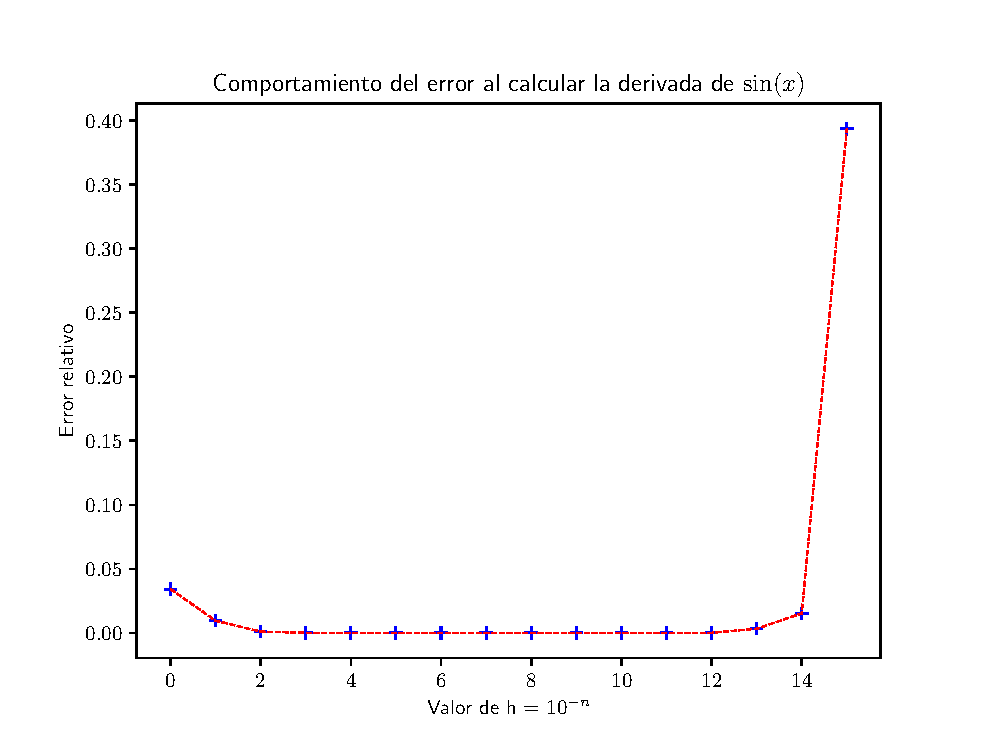
\includegraphics[scale=0.6]{Imagenes/Ejercicio_Derivada_00.eps}
\end{figure}
\end{frame}
\begin{frame}[fragile]
\frametitle{Ajuste de eje en la gráfica}
Vemos que hay un comportamiento de cambio drástico con los valores del error relativo, donde en apariencia el error relativo se cancela.
\\
\bigskip
\pause
Si ajustamos el eje $y$ a una escala logarítmica, quizá encontremos un resultado interesante.
\end{frame}
\begin{frame}[fragile]
\frametitle{Ajustando el eje $y$}
La siguiente instrucción nos presenta el eje $y$ en escala logarítmica:
\begin{verbatim}
plt.yscale('log')
\end{verbatim}
\end{frame}
\begin{frame}
\frametitle{Comportamiento del ER en escala semilog}
\begin{figure}
	\centering
    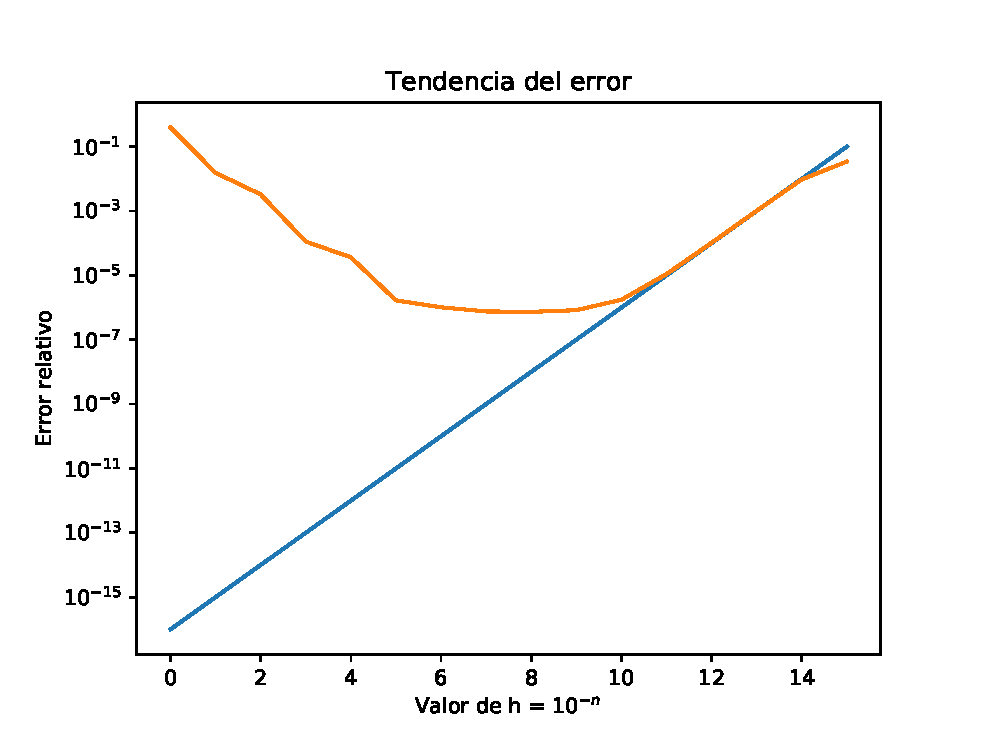
\includegraphics[scale=0.55]{Imagenes/Ejercicio_Derivada_01.eps}
\end{figure}
\end{frame}
\begin{frame}
\frametitle{Respuesta a la pregunta}
Si analizamos en detalle, vemos que la tendencia del error de truncamiento es lineal (en escala logarítmica) pero para $h < 10^{-8}$ el error aumenta y no sigue una ley determinada. 
\end{frame}
\begin{frame}
\frametitle{Respuesta a la pregunta}
Este \enquote{empeoramiento} de la aproximación se debe a la incidencia del error de redondeo, es decir, la unidad de máquina pasa a ser más importante que el error de truncamiento.
\end{frame}
\begin{frame}
\frametitle{Respuesta a la pregunta}
Es por eso que no siempre el utilizar una \enquote{mejor precisión} ayuda a mejorar los resultados finales. 
\\
\bigskip
En este tipo de problemas, es conveniente que el error que domine los cálculos sea el de truncamiento o de discretización.
\end{frame}



% \subsection{El código con \python}

% \begin{frame}[fragile]
% \frametitle{Estructuramos el código en \python.}
% Definimos mediante dos listas:
% \setbeamercolor{item projected}{bg=blue!70!black,fg=yellow}
% \setbeamertemplate{enumerate items}[circle]
% \begin{enumerate}[<+->]
% \item Los valores donde queremos evaluar el polinomio $P(x)$.
% \item Los coeficientes de $P(x)$.
% \end{enumerate}
% \begin{lstlisting}[style= FormattedNumber, basicstyle=\linespread{0.9}\ttfamily\normalsize, columns=fullflexible]
% # Valores de x0 para evaluar P(x0)
% x0=[-1.5, -0.65, 0.1, 1.4, 2.87]

% # Coeficientes a de P(x)
% a=[2,4,-5,2,-6,8,10]
% \end{lstlisting}
% \end{frame}
% \begin{frame}[fragile]
% \frametitle{Definimos una función que resuelva por Horner.}
% \fontsize{14}{14}\selectfont
% \begin{lstlisting}[style= FormattedNumber, basicstyle=\linespread{0.9}\ttfamily\normalsize, columns=fullflexible]
% # Metodo de Horner

% def P_Horner(x):
%     P_Hor=0
%     for n in range(len(a)-1,-1,-1):     
%         P_Hor=a[n]+P_Hor*x
%     return P_Hor
% \end{lstlisting}
% \end{frame}
% \begin{frame}[fragile]
% \frametitle{Definimos una función que evalúe directamente $P(x)$.}
% \fontsize{14}{14}\selectfont
% \begin{lstlisting}[style= FormattedNumber, basicstyle=\linespread{0.9}\ttfamily\normalsize, columns=fullflexible]
% # Evaluacion directa

% def P_Directo(x):
%     return 2+4*x-5*x**2+2*x**3-6*x**4+8*x**5+10*x**6
    
% \end{lstlisting}
% \end{frame}
% \begin{frame}[fragile]
% \frametitle{Calculamos el error relativo.}
% \fontsize{14}{14}\selectfont
% \begin{lstlisting}[style= FormattedNumber, basicstyle=\linespread{0.9}\ttfamily\normalsize, columns=fullflexible]
% # Calculo de error relativo

% def Err_Rel(p,p_): return (p-p_)/p*100
% \end{lstlisting}
% \end{frame}
% \begin{frame}[fragile]
% \frametitle{Mostramos el error relativo de los puntos a evaluar.}
% \fontsize{14}{14}\selectfont
% \begin{lstlisting}[style= FormattedNumber, basicstyle=\linespread{0.9}\ttfamily\normalsize, columns=fullflexible]
% # Evaluacion de valores de P(x0)

% for i in range(len(x0)):                 
%     print ("P(%.2f) =" %x0[i],P_Horner(x0[i]), "; Error rel. =", Err_Rel(P_Directo(x0[i]),P_Horner(x0[i])))
% \end{lstlisting}
% \end{frame}
% \begin{frame}[fragile]
% \frametitle{Comparamos los resultados con una gráfica.}
% \fontsize{14}{14}\selectfont
% \begin{lstlisting}[style= FormattedNumber, basicstyle=\linespread{0.9}\ttfamily\small, columns=fullflexible]
% import matplotlib.pyplot as plt
% import numpy as np

% x=np.linspace(-2.,3.)

% plt.plot(x,P_Horner(x),'ro', label='Metodo de Horner')

% plt.plot(x,P_Directo(x), label='Evaluacion Polinomio')

% plt.title('Comparacion grafica')
% plt.legend(loc='upper left')

% plt.grid(True)
% plt.show()
% \end{lstlisting}
% \end{frame}


\end{document}